\documentclass{article}
\usepackage{mainPoly}

\title{Généralités sur les fonctions}
\author{Seconde 9}
\date{}

\begin{document}
\maketitle

\section{Définitions}
\begin{tcolorbox}
\begin{definition}
Une \textbf{fonction} est un objet mathématique capable d'associer un \textbf{unique} résultat à tout objet d'un ensemble appelé \textbf{ensemble de définition}. 
\end{definition}
\end{tcolorbox}
\begin{example}
On définit plusieurs fonctions dont l'ensemble de définition est \emph{l'ensemble des élèves de la seconde 9} :
\begin{itemize}
\item $f$ est la fonction qui à un élève de la seconde 9 associe sa date d'anniversaire.
\item $g$ est la fonction qui à un élève de la seconde 9 associe sa couleur préférée.
\item $h$ est la fonction qui à un élève de la seconde 9 associe l'initiale d'un des membres de sa famille. \textbf{(Attention ! A-t-on vraiment défini une fonction ici ?)}
\item $p$ est la fonction qui à un élève de la seconde 9 associe \answersline
\item $q$ est la fonction qui à un élève de la seconde 9 associe \answersline
\end{itemize}
\end{example}
\begin{remark}
On s'intéresse majoritairement en mathématiques aux fonctions numériques. Les ensembles de définitions sont des ensembles de nombres, et le résultat renvoyé par les fonctions est toujours un nombre réel.
\end{remark}
\begin{tcolorbox}
\begin{definition}
Une \textbf{fonction numérique à valeurs réelles} est une fonction $f$ définie de la manière suivante :
\begin{equation*}
\function{f}{I}{\R}{x}{f(x)}
\end{equation*}
avec $I$ son \textbf{ensemble de définition}.
\end{definition}
\end{tcolorbox}
\begin{remark}
\hfill
\begin{itemize}
\item La plupart du temps, on aura $I = \R$, $I$ est un intervalle ou $I$ est une réunion d'intervalles.
\item On aura toujours $\R$ à droite de la flèche du haut : on dit que \textbf{l'ensemble d'arrivée} est $\R$.
\item La flèche du bas se lit de la manière suivante : au nombre $x$, on renvoie le nombre $f(x)$
\end{itemize}
\end{remark}
\begin{tcolorbox}
\begin{definition}
Soit $\function{f}{I}{\R}{x}{f(x)}$ et $a \in I$. On pose $b$ vérifiant l'égalité
\begin{equation*}
b = f(a)\,.
\end{equation*}
Alors, 
\begin{itemize}
\item $a$ est \textbf{un antécédent} de $b$ par la fonction $f$.
\item $b$ est \textbf{l'image} de $a$ par la fonction $f$.
\end{itemize}
\end{definition}
\end{tcolorbox}
\begin{example}
Soit $\function{f}{\R}{\R}{x}{2x+1}$.
\begin{enumquestions}
\item Donner l'image de $3$ par $f$ : \answersline
\item Donner un antécédent de $7$ par $f$ : \answersline
\end{enumquestions}
\end{example}
\newpage
\section{Courbe représentative}
\begin{tcolorbox}
\begin{definition}
Un \textbf{repère orthonormé} est un repère formé par deux axes tels que :
\begin{itemize}
\item Les deux axes sont perpendiculaires (on dit que le repère est \textbf{orthogonal})
\item Les deux axes sont gradués et ont des graduations de longueurs égales (on dit que le repère est \textbf{normé})
\end{itemize}
\end{definition}
\end{tcolorbox}
\begin{example} On représente traditionnellement un repère orthonormé de la manière suivante :
\begin{center}
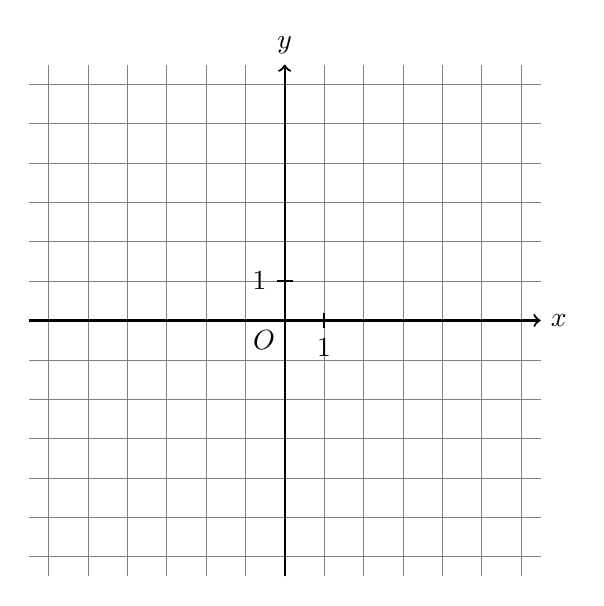
\begin{tikzpicture}
\draw[help lines] (-3.25,-3.25) grid[step=0.5] (3.25,3.25);
\draw[thick, ->] (-3.25,0) -- (3.25,0) node[right] {$x$};
\draw[thick, ->] (0,-3.25) -- (0,3.25) node[above] {$y$};
\draw (0,0) node[below left] {$O$};
\draw[thick] (0.5,0.1) -- (0.5,-0.1) node[below] {$1$};
\draw[thick] (0.1,0.5) -- (-0.1,0.5) node[left] {$1$};
\end{tikzpicture}
\end{center}
\begin{itemize}
\item L'axe horizontal est appelé \textbf{axe des abscisses}.
\item L'axe vertical est appelé \textbf{axe des ordonnées}.
\item Le point d'abscisse $0$ et d'ordonnée $0$ (de coordonnées $(0;0)$) est appelé \textbf{origine du repère}.
\end{itemize}
\end{example}
\begin{tcolorbox}
\begin{definition}
Soit $f$ une fonction définie sur un ensemble de définition $I$. On se place sur un reprère orthonormé. Alors, la \textbf{courbe représentative de $f$}, notée $\mathcal{C}_f$, est l'ensemble des points du repère de coordonnées $(x;y)$ vérifiant
\begin{equation*}
y = f(x)
\end{equation*}
\end{definition}
\end{tcolorbox}
\begin{remark}
La courbe représentative d'une fonction permet donc de représenter la fonction, c'est-à-dire de représenter la transformation d'un antécédent en une image par la fonction $f$. Chaque point de la courbe de coordonnées $(x;y)$ représente une telle transformation : l'abscisse $x$ du point joue le rôle de l'antécédent, et l'ordonnée $y$ du point joue le rôle de l'image.
\end{remark}
\begin{example}
Soit $f$ une fonction dont la courbe représentative est donnée sur le repère orthonormé suivant. Donner l'image de $3$ par $f$ : \answersline
\begin{center}
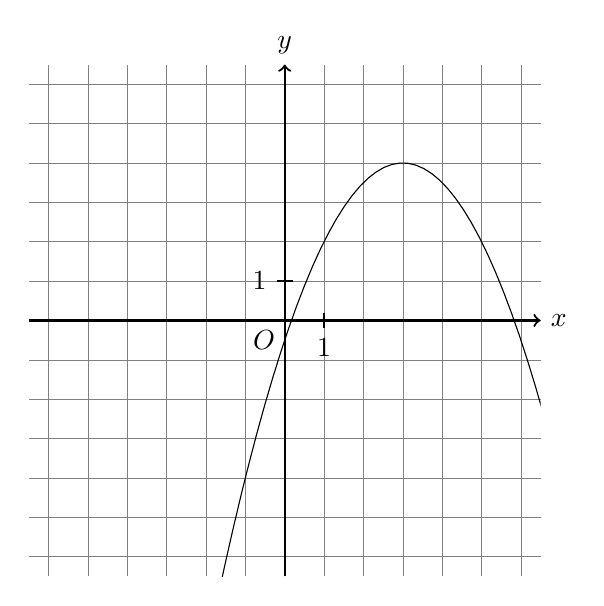
\begin{tikzpicture}
\draw[help lines] (-3.25,-3.25) grid[step=0.5] (3.25,3.25);
\draw[thick, ->] (-3.25,0) -- (3.25,0) node[right] {$x$};
\draw[thick, ->] (0,-3.25) -- (0,3.25) node[above] {$y$};
\draw (0,0) node[below left] {$O$};
\draw[thick] (0.5,0.1) -- (0.5,-0.1) node[below] {$1$};
\draw[thick] (0.1,0.5) -- (-0.1,0.5) node[left] {$1$};
\clip (-3.25,-3.25) rectangle (3.25,3.25);
\draw[samples=100] plot (\x,{-(\x-1.5)*(\x - 1.5) + 2});
\end{tikzpicture}
\end{center}
\end{example}

\end{document}